\documentclass{beamer}

\usetheme{Copenhagen}
\usepackage[utf8]{inputenc}
\usepackage{graphics}

% Slayt basliklarinda kullanilan font boyutu
\setbeamerfont{frametitle}{size=\normalsize}

\title{Kamera}
\author{Nurettin Şenyer}
\date{Şubat, 2011}
\institute[2011]{19/x}

\begin{document}

\frame{\titlepage}

\frame {
	\frametitle {Nasıl görürüz?}

	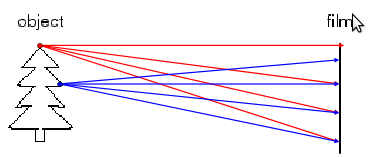
\includegraphics[width=0.90\textwidth]{img/02.png}

	Gözden hareketle kamera inşa edelim

	\begin{itemize}
		\item nesnenin önüne bir film koymak akla gelen ilk yoldur

		\item makul bir görüntü oluşur mu?

		\item Neden? \pause Nesnedeki tek noktadan çok sayıda ışık hüzmesi
		filmin farklı noktasına düşüyor

		\item \textbf{buğu} (blur) etkisi.

		\item hüzme fırçası
	\end{itemize}
}

\frame {
	\frametitle {Pinhole (iğne deliği) kamera}

	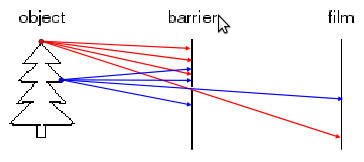
\includegraphics[width=0.90\textwidth]{img/03.png}

	Işık hüzmelerinin çoğunu engelleyen bir bariyer koyalım

	\begin{itemize}
		\item buğuyu azaltır

		\item bu delik (pinhole) - \textbf{açıklık} (aperture)

		\item tıp ki göz açıklığı - gözbebeği; diyafram

		\item ortaya çıkacak resim nasıldır? Nasıl oluşur?
	\end{itemize}
}

\frame {
	\frametitle {Pinhole (iğne deliği) kamera modeli}

	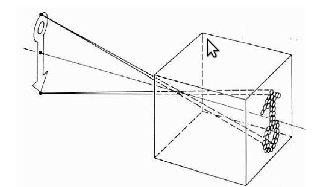
\includegraphics[width=0.70\textwidth]{img/04.png}

	Pinhole modeli,

	\begin{itemize}
		\item hüzme kalemi X fırçası - her bir hüzme tek bir noktadan/delikten
		geçer

		\item bu noktaya \textbf{Yansıma Merkezi} (COP - Center of Projection)
		denir

		\item resim, \textbf{Resim Düzlemi}'nden alınır

		\item Etkin odak uzunluğu - $f$, COP ile Resim Düzlemi arasındaki
		uzaklıktır

		\item dış dünya - analog X göz - ayrık/sayısal
	\end{itemize}
}

\frame {
	\frametitle {Boyut Azaltma Makinesi (3B den 2B ye}

	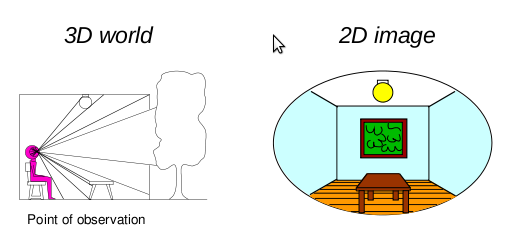
\includegraphics[width=0.90\textwidth]{img/05.png}

	Evinde sandalyesinde oturan kişinin gördüğü nedir? VEYA
	Kaybettiklerimiz nelerdir?

	\begin{itemize}
		\item açı
		\item mesafe (uzunluk)
	\end{itemize}
}

\frame {
	\frametitle {Eğlence ...}

	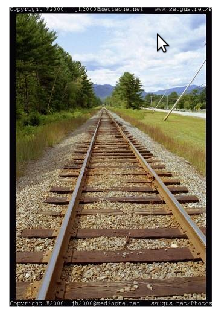
\includegraphics[height=0.90\textheight]{img/06.png}

	Uzaklık - yakınlık?
}

\frame {
	\frametitle {Paralel hatlar ne oldu?}

	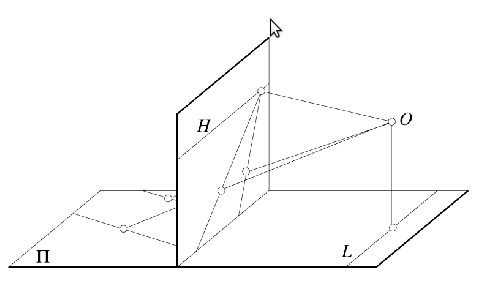
\includegraphics[width=0.90\textwidth]{img/07.png}

	Demiryolu (3B), kamera/resimde uzakta/sonsuzda tek noktada birleşiyor (2B)
}

\frame {
	\frametitle {Mesafelere ne oldu?}

	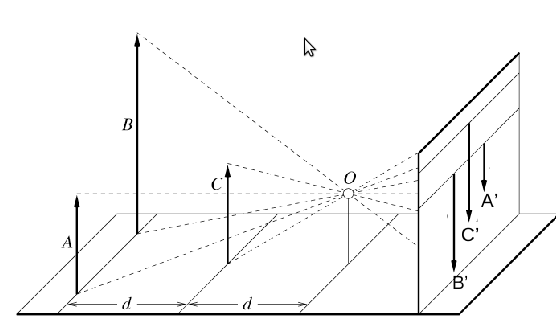
\includegraphics[width=0.90\textwidth]{img/08.png}

	3B den 2B ye geçilirken, farklı uzaklıktaki nesneler tek düzlemde
	gösterilmek zorunda
}

\frame {
	\frametitle {İnsanoğlu uyum sağlar}

	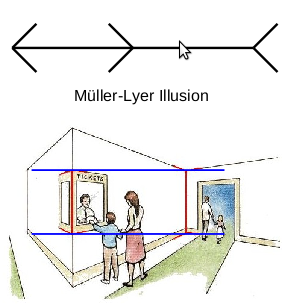
\includegraphics[width=0.90\textwidth]{img/09.png}

	\begin{itemize}
		\item 2B: aynı X 3B: farklı - yükseklik

		\item 2B: farklı X 3B: aynı - yükseklik
	\end{itemize}
}

\frame {
	\frametitle {Yansımayı Modelleme}

	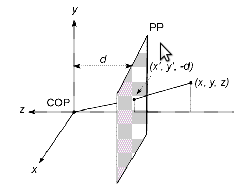
\includegraphics[width=0.90\textwidth]{img/10.png}

	Koordinat sistemi

	\begin{itemize}
		\item yaklaşımımız pinhole modeli

		\item orjin, optik merkezdedir (COP, Center Of Projection)

		\item görüntü düzlemi, COP'un önünde

		\item ::: Neden? \pause tersleyip - terslememe

		\item kamera negatif z eksenine doğru bakıyor
	\end{itemize}
}

\frame {
	\frametitle {Yansımayı Modelleme}

	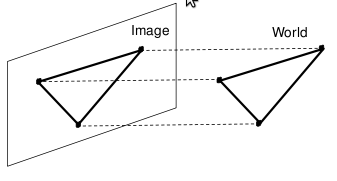
\includegraphics[width=0.90\textwidth]{img/14.png}

	Yansıma eşitlikleri

	\begin{itemize}
		\item $(x,y,z)$'den COP'a giden hüzmenin PP (resim düzlemi) ile kesişimi

		\item üçgen benzerliğinden

			$(x,y,z) \rightarrow (-d\frac{x}{z}, -d\frac{y}{z}, -d)$

		\item $d$ sabit olduğundan 3B'den 2B'ye geçebiliriz,

			$(x,y,z) \rightarrow (-d\frac{x}{z}, -d\frac{y}{z})$
	\end{itemize}
}

\frame {
	\frametitle {Homojen Koordinatlar}

	\begin{itemize}
		\item doğrusal bir dönüşüm müdür?

		\item ::: hayır - $z$ ile bölme, nonlinear

		\item ekstra bir koordinat ekle ($d = 1$ durumu)

		\item homojen \textbf{resim} koordinatları,

			$(x,y) \Rightarrow [x y 1]'$

		\item homojen \textbf{sahne} koordinatları,

			$(x,y,z) \Rightarrow [x y z 1]'$

		\item ters dönüşüm

			$(x,y,w) \Rightarrow (x/w, y/w)$

		\item ve benzer biçimde

			$(x,y,z,w) \Rightarrow (x/w, y/w, z/w)$

	\end{itemize}
}

\frame {
	\frametitle {Perspektif Yansıma}

	Yansıma, homojen koordinatların kullanıldığı çarpma matrisidir

	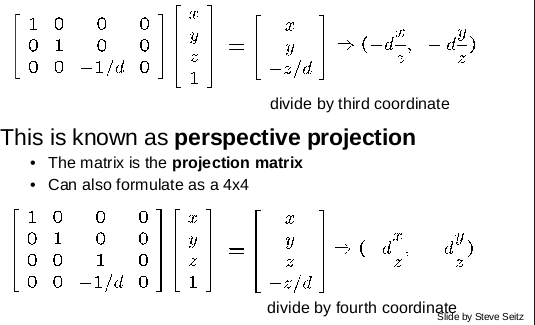
\includegraphics[width=0.90\textwidth]{img/13.png}
}

\frame {
	\frametitle {Dikçizgisel Yansıma}

	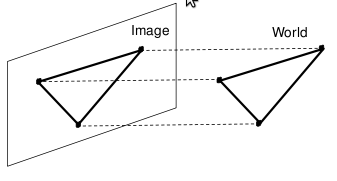
\includegraphics[width=0.75\textwidth]{img/14.png}

	Perspektif yansımanın özel durumu,

	\begin{itemize}
		\item COP - PP uzaklığı sonsuzdur

		\item "paralel yansıma" olarak da bilinir

		\item yansıma matrisi
			TODO
	\end{itemize}
}

\frame {
	\frametitle {Küresel yansıma}

	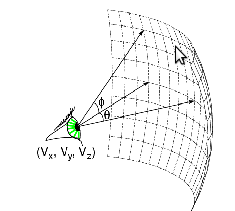
\includegraphics[width=0.65\textwidth]{img/15.png}

	\begin{itemize}
		\item PP, eğer COP'ta merkezli küreyse ne olacak?

		\item küresel koordinatlarda, yansıma

			$(\theta, \phi) = (\theta, \phi, d$

		\item ve odak uzaklığı temelli -$d$ bağımsızdır
	\end{itemize}
}

\frame {
	\frametitle {Gerçek Kamera}

	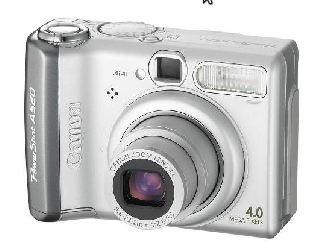
\includegraphics[width=0.90\textwidth]{img/16.png}
}

\frame {
	\frametitle {İlk Kamera}

	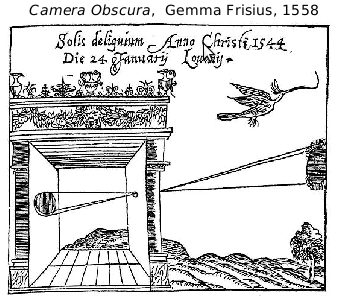
\includegraphics[width=0.90\textwidth]{img/17.png}

	İlk kamera

	\begin{itemize}
		\item Aristo: kağıt üzerine düşürülüyor

		\item oda derinliği, etkin odak uzunluğu
	\end{itemize}
}

\frame {
	\frametitle {Ev yapımı pinhole kamera}

	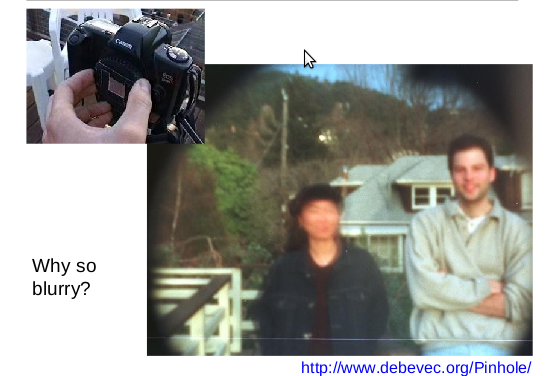
\includegraphics[width=0.90\textwidth]{img/18.png}
}

\frame {
	\frametitle {Aperturu daraltma}

	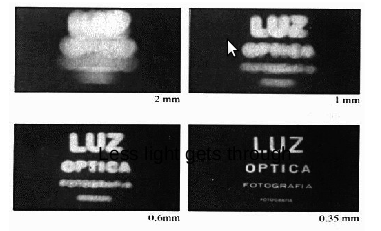
\includegraphics[width=0.90\textwidth]{img/19.png}

	(pinhole çapının küçülmesi: `2 mm` - `0.35 mm`)

	Aperturu olabilecek en küçük neden yapamayız?

	\begin{itemize}
		\item daha ışık girer

		\item saçınım etkisi
	\end{itemize}
}

\frame {
	\frametitle {Aperturu daraltma}

	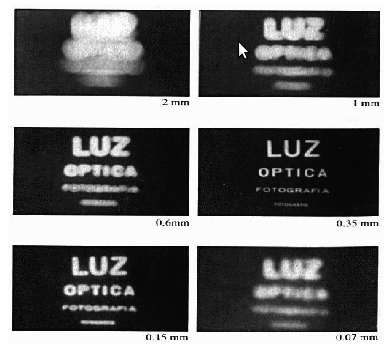
\includegraphics[width=0.90\textwidth]{img/20.png}
}

\frame {
	\frametitle {Aperturu daraltma}

	x: pinhole çapı, y: görsel kalite

	\begin{itemize}
		\item x küçüldükçe az ışık ve saçınım etkisi
		\medskip

		\item x büyüdükçe buğu etkisi
		\medskip

		\item x = x0 = `0.35 mm` oldukça iyi sonuç üretiyor (global maximum)
	\end{itemize}
}

\frame {
	\frametitle {Neden lens kullanılır?}

	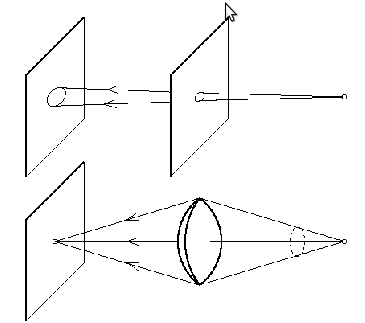
\includegraphics[width=0.90\textwidth]{img/21.png}

	Sol taraf: 2B, orta: COP ve sağ taraf: 3B'dir. Lens odaklar.
}

\frame {
	\frametitle {Neden lens kullanılır?}

	ODAKLAMA
}

\frame {
	\frametitle {Lens yardımıyla resmi oluşturma}

	İdeal Lens: pinhole ile aynı yansıma fakat daha fazla ışıkla!

	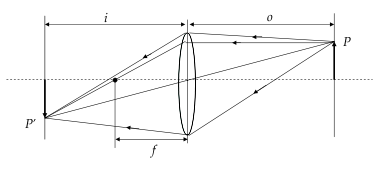
\includegraphics[width=0.50\textwidth]{img/23.png}

	(sol taraf: perde/2B/PP, sağ: 3B)

	Lens formülü: $\frac{1}{i} + \frac{1}{o} = \frac{1}{f}$

	\begin{itemize}
		\item $f$, lensin odak uzaklığıdır - ışık kırma yeteneği

		\item $f$, etkin odak uzunluğu-$f$'den farklıdır!

		\item Hatır: "etkin odak uzaklığı" COP - PP arası uzaklıktı

		\item $f$, COP - lens arası mesafe
	\end{itemize}
}

\frame {
	\frametitle {Lens yardımıyla resmi oluşturma}

	\begin{itemize}
		\item ya perdeyi

		\item ya ada lensi hareket ettir

		\item hareket: sağ-sol
	\end{itemize}
}

\frame {
	\frametitle {Odaklama - odaktan uzaklaşma}

	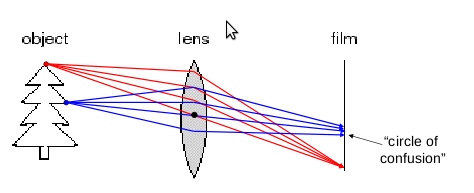
\includegraphics[width=0.90\textwidth]{img/22.png}

	Lens, ışığı film üzerine odaklar

	\begin{itemize}
		\item nesnelerin odaklanmasında belli bir mesafe vardır

		\item ::: bu mesafedikler odaklıdır

		\item ::: diğerlerinin odağı bozuktır

		\item ::: bu "çakışma çemberi" olarak karşımıza çıkar

		\item odak mesafesini nasıl değiştirebiliriz?
	\end{itemize}
}

\frame {
	\frametitle {Odaklama - odaktan uzaklaşma}

	\begin{itemize}
		\item pinhole'de tek ışın geçiyordu

		\item lensle çok sayıda ışın geçiyor

		\item tek noktaya odaklanıyor - "in focus"

		\item daireye odaklanıyor - "defocus"
	\end{itemize}
}

\frame {
	\frametitle {İnce Lens}

	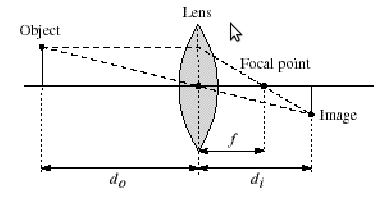
\includegraphics[width=0.90\textwidth]{img/24.png}

	İnce lens eşitliği: $\frac{1}{d_o} + \frac{1}{d_i} = \frac{1}{f}$

	\begin{itemize}
		\item bu eşitliği sağlayan nesne noktaları odaklıdır

		\item odak bölgesinin şekli nedir?

		\item odak bölgesini nasıl değiştirebiliriz?

		\item ince lens applet: $http://www.phy.ntnu.edu.tw/java/Lens/lens_e.html$ (by
		Fu-Kwun Hwang)
	\end{itemize}
}

\frame {
	\frametitle {Alan Derinliği (DOF: Depth of Field)}

	ALAN DERİNLİĞİ
}

\frame {
	\frametitle {Alan Derinliği (Depth of Field)}

	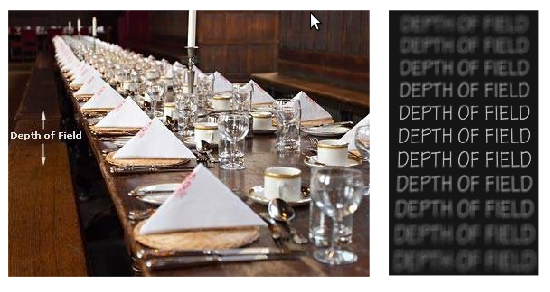
\includegraphics[width=0.90\textwidth]{img/27.png}
}

\frame {
	\frametitle {Alan Derinliği (Depth of Field)}

	\begin{itemize}
		\item alttan-yukarı dernilik artıyor

		\item odaklanan (orta bölge) net

		\item gerisi (gerek yakın gerekse uzak) bulanık

		\item buna derinlik etkisi deniyor
	\end{itemize}
}

\frame {
	\frametitle {Aperturla Derinlik Etkisi Denetleme}

	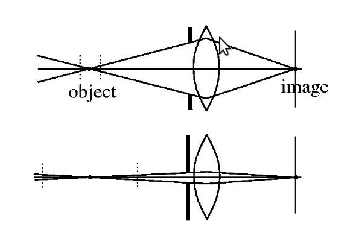
\includegraphics[width=0.90\textwidth]{img/28.png}

	(üsttekinde pinhole geniş, alttakinde dar)

	Apertur boyutunu değiştirmek alan derinliğini etkiler

	\begin{itemize}
		\item apertur küçüldükçe, odaklı nesne erimi artar
			  % daha fazla nesne odaklanmış olur

		\item fakat ışık azalır, pozlama süresini artırmak gerekir
	\end{itemize}
}

\frame {
	\frametitle {Aperturu değiştirmek}

	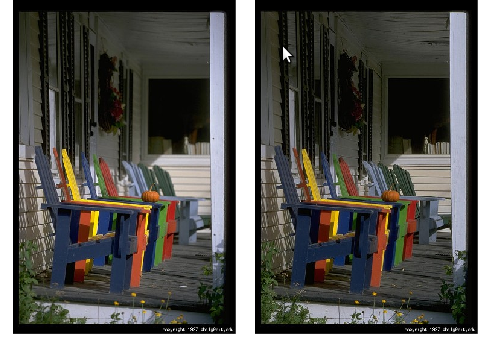
\includegraphics[width=0.90\textwidth]{img/29.png}

	(sol: büyük apertur=dar DOF, sağ: küçük apertur=geniş DOF)

	Balkabağına odaklanılmış, gerisi az veya çok buğulu
}

\frame {
	\frametitle {Güzel bir DOF örneği}

	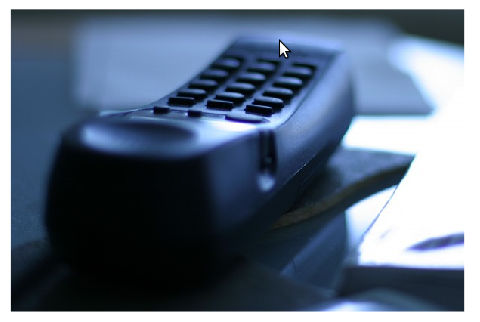
\includegraphics[width=0.90\textwidth]{img/30.png}
}

\frame {
	\frametitle {Görüş Sahası (FOV: Field Of View)}

	ALAN DERİNLİĞİ (zoom)
}

\frame {
	\frametitle {Alan Derinliği odak uzunluğuna bağlıdır}

	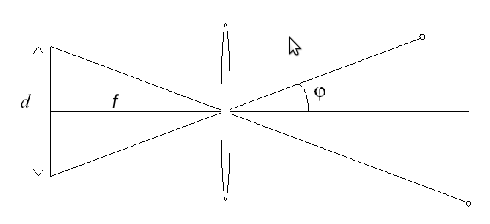
\includegraphics[width=0.90\textwidth]{img/34.png}

	(sol: PP, orta: lens/mercek, sağ: nesne; f = PP-lens arası mesafe)

	FOV'un boyutu, kamera retinasının boyutuyla belirlenir

		$\phi = tan^{-1}(\frac{d}{2f})$

	Buradaki $\phi$ görüşün yapıldığı açıklığın açısıdır

	FOV küçükse = odak uzaklığı büyüktür

	Mercek hareket ettirilerek nesneye zoomlanabilir
}

\frame {
	\frametitle {Perspektif}

	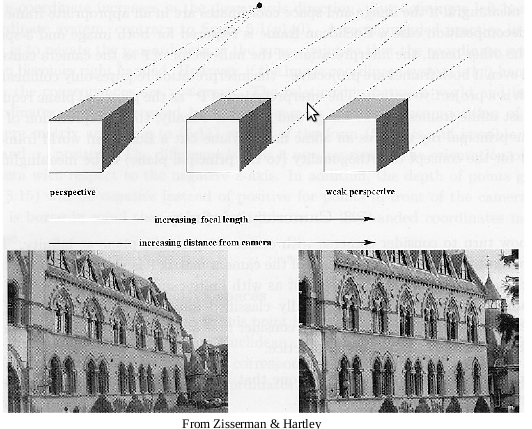
\includegraphics[width=0.90\textwidth]{img/35.png}
}

\frame {
	\frametitle {FOV / Odak Uzaklığı}

	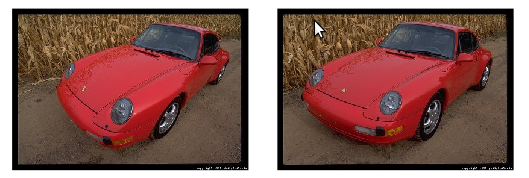
\includegraphics[width=0.90\textwidth]{img/36.png}

	\begin{itemize}
		\item AYNI görünümlü resimlerden

		\item Sol: büyük FOV, kısa $f$, kamera arabaya daha yakın

		\item Sağ: küçük FOV, uzun $f$, kamera arabaya uzak
	\end{itemize}
}

\frame {
	\frametitle {Odak Uzaklığı - Oyun Sektörü}

	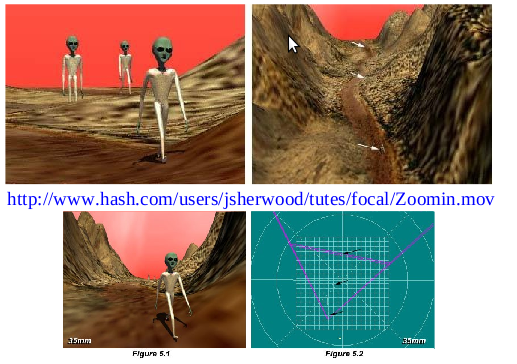
\includegraphics[width=0.90\textwidth]{img/37.png}
}

\frame {
	\frametitle {Lens Kusurları}

	LENS KUSURLARI
}

\frame {
	\frametitle {Lens Kusurları: renge bağlı sapma farklılıkları}

	Saçılma: dalgaboyuna bağlı kırılma indisi

	\begin{itemize}
		\item prizmanın beyaz ışıktan renk şeriti/gökkuşağını çıkartması
	\end{itemize}

	Odak uzaklığı dalga boyuyla değişir: $f(\lambda)$

	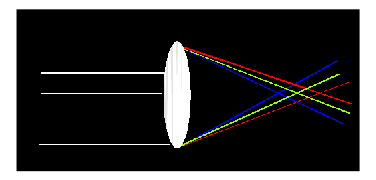
\includegraphics[width=0.90\textwidth]{img/39.png}

	\begin{itemize}
		\item resmin kenarlarında renkli saçaklar oluşur

		\item düzeltme: kristal çift lens kullanımı

		\item düzeltme: her bir renge (RGB) farklı muamele
	\end{itemize}
}

\frame {
	\frametitle {Renge bağlı Bozulma}

	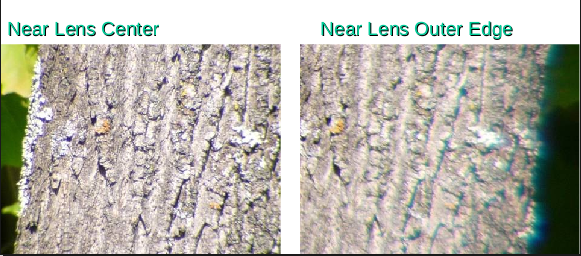
\includegraphics[width=0.90\textwidth]{img/40.png}
}

\frame {
	\frametitle {Işınsal/radyal Bozulma}

	'Fıçı' ve 'iğne-yastığı' bozulması

	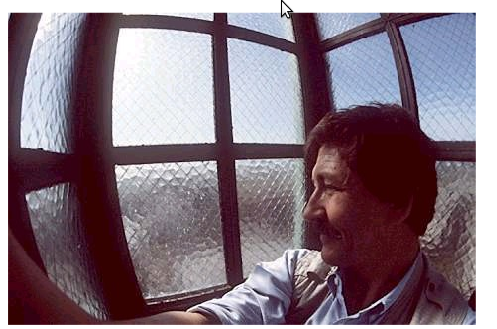
\includegraphics[width=0.90\textwidth]{img/41.png}

	Düz çizgiler, merkez etrafında eğrilir
}

\frame { 
	\frametitle {Işınsal Bozulma} 
	
	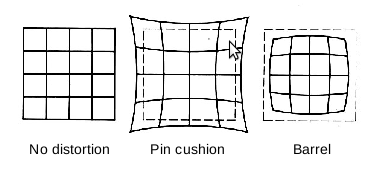
\includegraphics[width=0.90\textwidth]{img/42.png}
	
	(Sol: bozulma yok, orta: yastık, sağ: fıçı)

	resimde ışınsal bozulma

	\begin{itemize}
		\item lens mükemmelsizliklerinden kaynaklıdır

		\item sapmalar, en fazla kenarlarda fark edilir

		\item fıçı: büyük kürenin küçük bir dilimi

		\item TV:sony:silindir
	\end{itemize}
}
\frame { 
	\frametitle {Işınsal Bozulma} 
	
	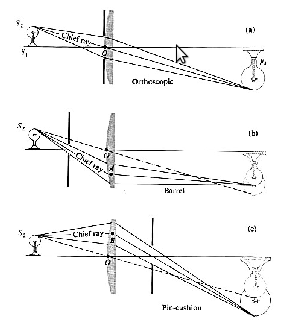
\includegraphics[width=0.90\textwidth]{img/43.png}

	(lens sabit, açıklık hareketli, farklı bozulma etkileri)
}

\frame {
	\frametitle {Işınsal Bozulma}

	Demo: $http://mw.cmla.ens-cachan.fr/megawave/demo/lens_distortion$

	Demo: site.gif, demo.gif
}

\end{document}
